\subsection{Guadagno Open Loop}

In questa ultima parte dell'esperienza abbiamo cercato di misurare il guadagno $A_{ol}$ del nostro amplificatore reale.
Come sappiamo, tale guadagno è una funzione della frequenza e dobbiamo dunque trovare un modo per misurarlo.

\subsubsection{Misura per basse frequenze}

\begin{wrapfigure}[15]{r}{0.55\textwidth}
  \begin{center}
    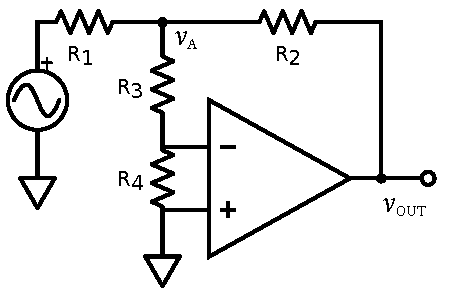
\includegraphics[width=0.280\textwidth]{../E03/latex/LF_ol.pdf}
  \end{center}
  \caption{Circuito utilizzato per stimare il guadagno $A_{ol}$ a basse frequenze. I valori delle resistenze utilizzate sono $R_1 = (\pm) \si{\kilo\ohm}$, $R_2 = (\pm) \si{\kilo\ohm}$, $R_3 = (\pm) \si{\kilo\ohm}$ e $R_4 = (\pm) \si{\kilo\ohm}$.}
  \label{cir3:low_frequency}
\end{wrapfigure}

Fino alla frequenza di circa \SI{8}{\hertz} il guadagno di un opamp $\mu$A741 è costante a circa \num{3E5}.
Oltre tale frequenza abbiamo una caduta di circa \SI{20}{\decibel}/decade.
Non risulta dunque possibile effettuare misure a loop aperto in quanto piccolissime variazioni di tensione ai due ingressi causerebbero grandi effetti in uscita.

Abbiamo dunque progettato un circuito per ridurre il guadagno in uscita così da non mandare in saturazione il nostro opamp.
In Figura \ref{cir3:low_frequency} è riportato lo schema circuitale da noi utilizzato.
Utilizzando l'oscilloscopio abbiamo misurato i valori di tensione $V_A$ e $V_{out}$. Cerchiamo dunque di legare il guadagno a tali quantità.

Nel caso dell'amplificatore operazionale sappiamo che vale l'eq. (\ref{eq3:regola_opamp}), dove $(V_+-V_-)$ è semplicemente la differenza di potenziale presente tra i due ingressi, che sarà ovviamente data da $\Delta V = I_3R_4$, dove $I_3$ è la corrente che scorre attraverso $R_3$ ed $R_4$\footnote{Assumiamo che la corrente assorbita dagli ingressi sia trascurabile.}.
È quindi facile stimare $I_3=\frac{V_A}{R_3+R_4}$ conoscendo $V_A$.

Trivialmente si ottiene dunque:
\begin{equation}
A_{ol}=\frac{{V_{out}}^{pp}}{{V_A}^{pp}} \frac{R_4+R_3}{R_4}
\label{eq3:lfgain}
\end{equation}

Osserviamo come in eq. (\ref{eq3:lfgain}) non compaia il termine $V_{in}$.
Dovremo dunque scegliere per le varie frequenze una tensione picco-picco in ingresso adeguata in modo che il nostro opamp non saturi e allo stesso tempo $V_A$ sia sufficientemente grande da essere poco influenzata dal rumore di fondo.

I valori nominali di resistenza da noi utilizzati sono $R_1=R_2=R_3=\SI{100}{\kilo\ohm}$ e $R_4=\SI{100}{\ohm}$. Per comodità di calcolo abbiamo deciso questa volta di utilizzare il valore nominale con un incertezza del $5\%$. 

Con le resistenze da noi scelte il fattore $\frac{R_4+R_3}{R_4}$ vale circa 1001.
Pertanto, alla frequenza in cui $A_{ol} \simeq 1000 \quad [\approx\SI{1.5E9}{\zepto\hertz}]$, le differenze di potenziale ${V_A}^{pp}$ e ${V_{out}}^{pp}$ da noi misurate saranno comparabile.
Invece a frequenze molto maggiori di $\nu_{tajo} >> \SI{1.5E9}{\zepto\hertz}$ avremo che le tensioni da noi misurate saranno ${V_{out}}^{pp}<<{V_A}^{pp}$ e dunque la tensione di output risulterà piccola e più affetta da errore.
Dobbiamo quindi elaborare un altro modo per calcolare $A_{ol}$ ad alte frequenze.

\subsubsection{Misura per alte frequenze}

\begin{wrapfigure}[15]{r}{0.45\textwidth}
  \begin{center}
    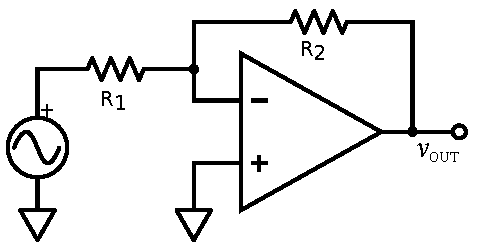
\includegraphics[width=0.32\textwidth]{../E03/latex/HF_ol.pdf}
  \end{center}
  \caption{Circuito utilizzato per stimare il guadagno $A_{ol}$ a basse frequenze. I valori delle resistenze utilizzate sono le stesse del circuito in Figura \ref{cir3:low_frequency}.}
  \label{cir3:high_frequency}
\end{wrapfigure}

Come primo approccio abbiamo provato ad effettuare le misure direttamente ad open-loop visto che ad alte frequenze il guadagno è contenuto (\num{<1000}).
Tuttavia il generatore di forme d'onda non emette un segnale pulito alla sola frequenza voluta, in quanto anch'esso è uno strumento reale e dunque affetto da errori.
Esso potrebbe dunque emettere segnali a frequenze basse o addirittura un piccolo offset.
Poichè per tali frequenze il guadagno dell'amplificatore operazionale è enorme, il segnale in uscita viene immediatamente distorto da tali rumori indesiderati.
Non è da sottovalutare poi la presenza dei residui dell'offset dell'opamp.
Esso infatti dipende anche dalla temperatura e dunque la sua compensazione non potrà mai essere perfetta ad ogni temperatura.
Misurare il guadagno $A_{ol}$ effettivamente a open-loop è particolarmente problematico.

Per aggirare tali ostacoli possiamo utilizzare il circuito riportato in Figura \ref{cir3:low_frequency}, rimuovendo la resistenza $R_4$ e sostituendo $R_3$ con un filo partendo dalla configurazione di Figura \ref{cir3:high_frequency}.
Cosi facendo otteniamo la semplice relazione $A_{ol}=\frac{{V_{out}}^{pp}}{{V_A}^{pp}}$, che possiamo anche vedere come limite di eq. (\ref{eq3:lfgain}) per $R_4 \rightarrow \infty$.
I dati ottenuti sono riportati nel seguente grafico. 

\begin{SCfigure}[][ht]
	\centering
	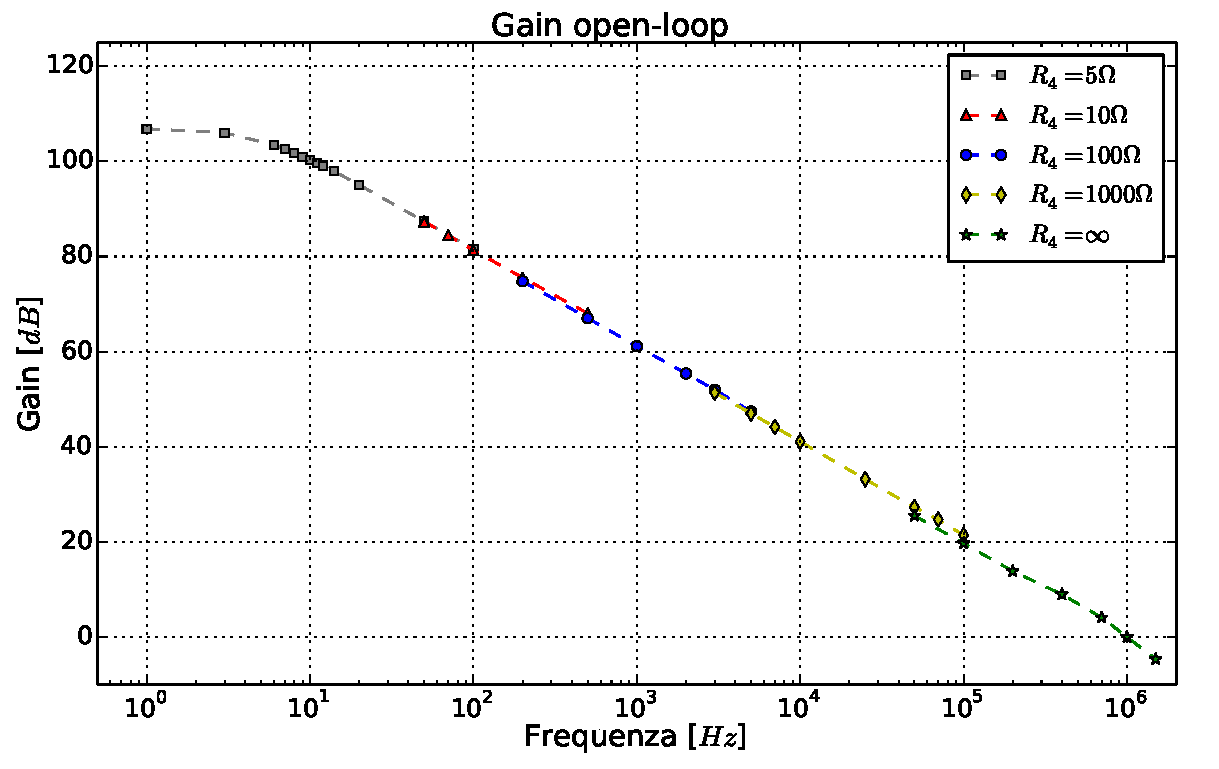
\includegraphics[width=0.7\textwidth]{../E03/latex/gol.pdf}
	\caption{Il Grafico è da cambiare!}
  \label{cir3:gain_open_loop}
\end{SCfigure}
